\documentclass{article}[18pt]
\usepackage{../../../../format}
\lhead{Software Methodologies - Computer Graphics}


\begin{document}
\begin{center}
\underline{\huge GPU Programming with WebGL}
\end{center}
\begin{definition}[Polygon model/mesh]
Comprises a set of connected polygons to represent an object
\end{definition}
\section{Why WebGL}
\begin{itemize}
	\item Cross-platform, browser-based
	\item Hardware-based rendering
	\item Support programmable rendering pipeline
	\item Zero setup effort before you start programming
\end{itemize}
\section{GPU Programming}
GPU
\begin{itemize}
	\item Typically comprises of hundreds to thousands of processors
	\item Process graphics primitives in parallel
\end{itemize}
Programmable rendering pipeline
\begin{itemize}
	\item Vertex shader and fragment shader are programmable
	\item GPU programming is also called shader programming
\end{itemize}
\section{Programmable rendering pipeline}
\begin{center}
	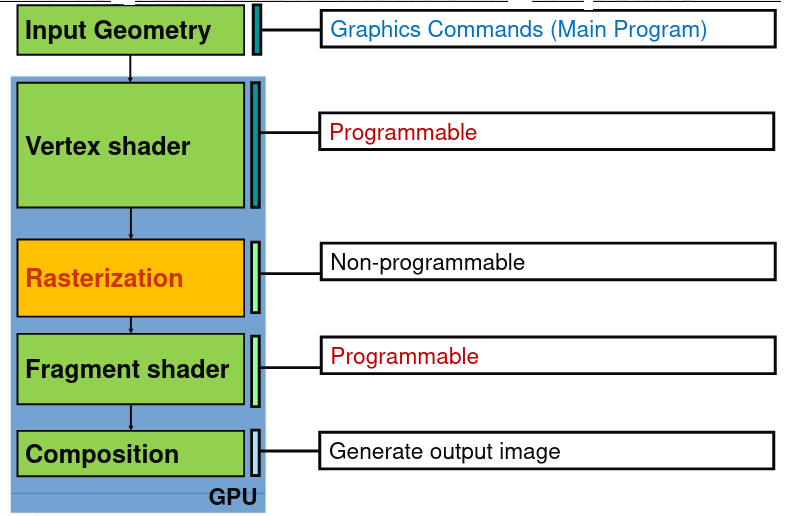
\includegraphics[scale=0.7]{pipeline}
\end{center}
Pixels - Colour info\\
Fragment - Single point with more information than a pixel, e.g.  lighting effects
\section{Shaders}
Vertex shader:
\begin{itemize}
	\item Manipulates per-vertex data such as vertex coordinates, normals, colors, and texture coordinates
\end{itemize}
Fragment shader:
\begin{itemize}
	\item Deals with surface points for processing
	\item Main goal: calculate colour for each pixel that will display on the screen
\end{itemize}
Rasterization process:
\begin{itemize}
	\item A black box (non programmable) generates fragments from outputs of vertex shader
\end{itemize}
\section{Data Structures}
\begin{definition}[Vertex Buffer Objects (VBOs)]
Contain the data that WebGL requires to describe the geometry that is going to be rendered
\end{definition}

\begin{definition}[Index Buffer Objects (IBOs)]
	Contain integers that use as references pointing to data in VBOs, in order to enable the reuse of the same vertex
\end{definition}

Attributes, uniforms and varyings are the three types of variables that you will find when programming with shaders
\begin{definition}[Attributes]
	Input variables used in the vertex shader (dynamic)
\end{definition}

\begin{definition}[Uniforms]
Input variables available for the vertex shader and the fragment shader (static)
\end{definition}

\begin{definition}[Varyings]
Used for passing data from the vertex shader to the fragment shader
\end{definition}








\end{document}